\paragraph{}
This chapter gives an overview about the general virtual machine, 
defines both tha Java programming language and the Java Virtual Machine. 
The chapter also contains information about embedded systems and the ARM
\footnote{Advanced RISC Machines } architecture that is the commonly used in embedded systems.
\section{What is a Virtual Machine?}
\paragraph{}
Virtual Machine, in general, is a software abstraction of a computer that often executes as a user application on top of the native operating system. One application of virtual machines is to allow multiple instances of an operating system to execute concurrently. Another is emulation using software or hardware that mimics the functionality of hardware or software not present in the system. In other words it promotes portability by decoupling the relation between program execution and the host environment or hardware design or both. Virtual machines interface with the hardware in a system via the underlying operating system, other user programs can interact with VMs. A VM can create software components that represent the content of physical systems such as processors, memory, communication channels, disks and clocks (see Figure~\ref{fig:VM}).


\begin{figure}[h]
\centering
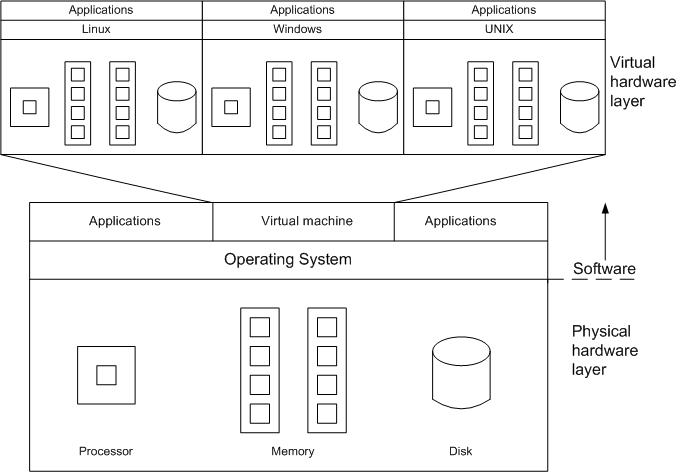
\includegraphics[width=0.9\textwidth,height=0.5\textheight]{vm.png}
%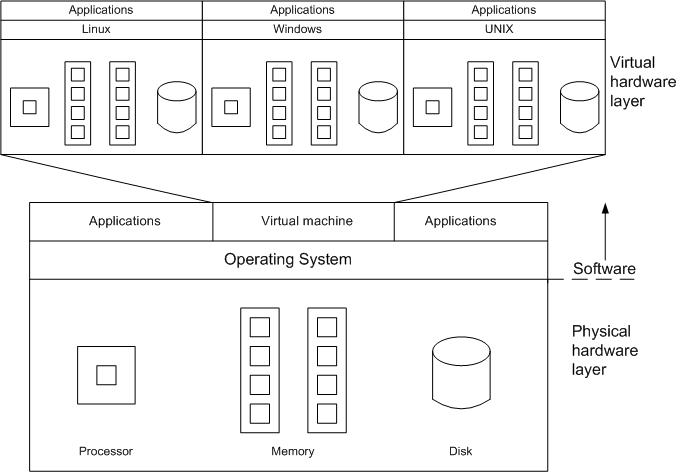
\includegraphics[]{vm.png}
\caption{Schematic of a Virtual Machine}
\label{fig:VM}
\end{figure} 

%the figure of the virtual machines
\paragraph{}
Early examples are the IBM VM, and Pascal p-Code machine. The VM was apparently the first true virtual machine system. It introduced the radical concept of a self-virtualizing processor instruction set. Essentially VM and the mainframe hardware cooperate so that multiple instances of any operating system, each with protected access to the full instruction set, can peacefully and concurrently coexist. This virtualization capability is so strong that VM can run as a guest inside itself even multiple levels deep without much performance penalty. The p-Code machine or pseudo-code machine \footnote{A p-code is similar to a byte-code (mentioned later) but a p-code works at a higher level. Whereas byte-codes work at a very low level similar to machine code, p-codes can perform moderately complex tasks such as printing a message or clearing the screen.} was the target of some early Pascal implementations. Pascal was translated not to machine code instructions (understandable directly to a processor) but to p-code instructions. To execute the program, another program is used that interprets this code.
\section{What is Java?}
\paragraph{}
Java\texttrademark Technology Introduced By Sun \footnote{Stanford University Network} Microsystems, Inc  with attractive Write Once, Run Anywhere concept where Java program is compiled into machine independent byte-code which is simple stack-based (i.e. not register-based) low level instructions in order to be easily interpreted by almost any hardware platform. Thus Java is a choice where heterogeneous platforms exist and need to communicate, which is the case for the World. Java faced criticism for performance \footnote{indeed optimized java code run by factor of 5 slower than corresponding C++ code. The C++ Complete Refrence, Osborne}, memory consumption, portability issues \footnote{need for native calls still exist but with every one following sun’s notation of the API it could be considered portable or part of the standard}, and not being FOSS (Free Open Source Software) \footnote{Java virtual machine standard is feely available but all implementation issues are proprietary licensed software}.Though, it has steadily evolved for several reasons first Processors having bursts of performance acceleration second, Memory getting faster and cheaper, allowing fast complex Technologies - like the HotspotTM- or JIT \footnote{Just In Time Compiler} to be adoptable.
\section{What is the Java Virtual Machine (JVM)}
\paragraph{}
The Java virtual machine (JVM) is an abstract computer or a machine within a machine. Its specification defines certain features every Java virtual machine must have, but leaves many choices to the designers of each implementation. The main job of the Java virtual machine is to execute Java bytecodes. The Java virtual machine specifications did not specify or restrict a certain execution technique that the Java virtual machine must follow. The flexible nature of the Java virtual machine's specification enables it to be implemented on a wide variety of computers and devices.
\section{The Class File and the Byte Code}%\cite{insideJVM}
\section{Embedded Systems}
\paragraph{}
Embedded Systems provide a different software design challenge. They are characterized by a small set of specialized resources that provide functionality to devices such as cell phones and PDAs (Personal Digital Assistant). In embedded environments, efficient resource management is the key to building successful software. One of the most important software design limitations that embedded systems provide is the storage limitation, the software must provides services using a minimal amount of code. Considerations such as power management and the need for user-friendly interfaces create other challenges in embedded software design.
\section{ARM Architecture}
\paragraph{}
ARM Architecture (Originally the Acorn RISC Machine currently Advanced RISC Machines) has become one of the most used CPU designs in the world, found in everything from hard drives, to mobile phones, to routers, to calculators, to children’s toys. Today it accounts for over 75\% of all 32-bit embedded CPU’s. That is for its low cost yet high performance advantage. ARM family reached ARM11 and is licensed to many companies IBM, Infineon Technologies, Texas Instruments, Nintendo, Philips, VLSI, Atmel, Sharp and Samsung.
%\section{Secure Execution}
\section{Conclusions}
The existence of the Java virtual machine is considered an important matter nowadays; 
especially for the embedded systems that are found in different architectures. 
The next chapter introduces the Java virtual machine's architecture in terms 
of its modules and subsystems.
